\chapter{Zastosowanie układów rekonfigurowalnych w bezzałogowych statkach powietrznych}

Drony są urządzeniami, które zazwyczaj pracują w pewnej odległości od osoby nadzorującej, a często nawet poza jej zasięgiem widzenia. 
O ile może rodzić to pewne trudności, jest to chociażby jeden z głównych powodów udziału dronów w zastosowaniach militarnych -- wówczas operator drona wojskowego nie tylko znajduje się poza obszarem zagrożenia, ale często zdalnie podejmowane przez niego decyzje wiążą się z niższym poziomem stresu. 
Taka platforma powietrzna musi być jednak wyposażona w elementy elektroniczne pozwalające przesłać użytkownikowi zestaw danych o statusie drona. 
Podstawową grupę pełnią informacje telemetryczne z czujników (akcelerometr, żyroskop, GPS, stan baterii lub zapas paliwa w zbiorniku). 
Ponadto, już nawet komercyjne drony ze średniej półki cenowej umożliwiają przesłanie informacji wizyjnej, a niektóre nawet ją przetwarzają. 
Przykładem może być DJI Spark, miniaturowa konstrukcja, która na podstawie informacji z wbudowanej kamery może wykonywać komendy wydawane gestami \cite{SPARK}.

Poprawne działanie platformy latającej wymaga przetworzenia sporej ilości informacji, gwałtownie rosnącej wraz z dodawaniem nowych funkcjonalności. 
Na etapie projektowania ważne jest zatem dobranie odpowiedniej jednostki obliczeniowej. 
Schemat \ref{fig:autopilot_architecture} opisuje podstawowe zależności w systemie, które należy uwzględnić definiując architekturę.
\begin{figure}[h]
	\centering
	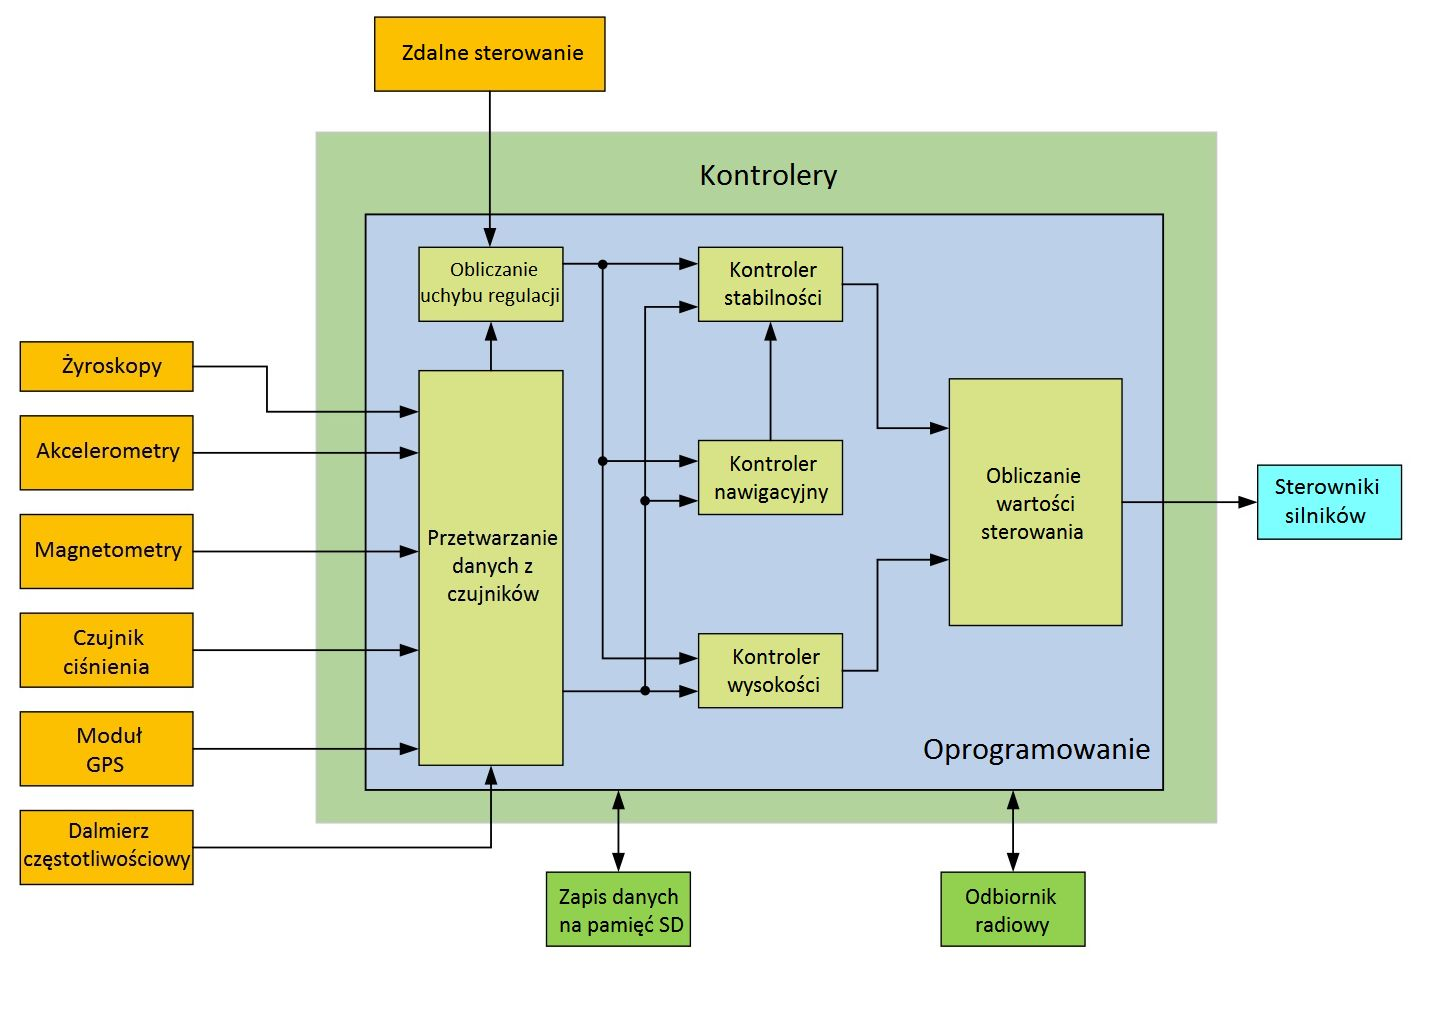
\includegraphics[width=12cm]{7_drone_platform_overview.jpg}
	\caption{Architektura programowo-sprzętowa związana z pracą autopilota \cite{Bouhali2017} }
	\label{fig:autopilot_architecture}
\end{figure} 

Rynek urządzeń typu UAV obfituje w rozwiązania oparte mikrokontrolery. 
Popularnymi autopilotami stosowanymi w komercyjnych produktach -- i przede wszystkim w ręcznie tworzonych konstrukcjach -- są: NAZA-M V2 firmy DJI oraz Pixhawk firmy 3DR. 
Oba te moduły, bazując na mikrokontrolerach ARM i dużej liczbie peryferiów, w zupełności wystarczają do zastosowań niewymagających przetwarzania dużej ilości danych, zapewniając łączność z aparaturą radiową i realizację misji opartych na predefiniowanej sekwencji ruchów. 

Nieco bardziej rozbudowane są rozwiązania wykorzystujące dwa mikrokontrolery -- jeden z~nich jest skonfigurowany w tzw. trybie „baremetal”, który oznacza uruchomienie aplikacji bezpośrednio na procesorze. 
Umożliwia to wykonywanie niskopoziomowych, krytycznych zadań, jak na przykład stabilizacja lotu uwzględniająca sterowanie pracą silników i pomiar wartości z czujników. 
Na drugim mikrokontrolerze uruchomiony jest system operacyjny, który stanowi platformę dla aplikacji wysokopoziomowych -- takich jak algorytmy planowania trasy, stereowizja czy śledzenie celu. 
Jedną z takich komercyjnych platform jest „MikroKopter” stworzony przez firmę HiSystems GmbH \cite{MikroKopter}.

Układy rekonfigurowalne, w miarę postępu technologicznego, stają się godną uwagi alternatywą -- pomimo często wyższej ceny oferują konkurencyjną wartość poboru mocy i niezrównanie szybszą prędkość działania algorytmów. 
Szczególnie, jeśli podczas ich implementacji uwzględni się możliwość zrównoleglania obliczeń. 

\section{Układy rekonfigurowalne w roli autopilota platformy UAV}

Przewaga układów rekonfigurowalnych okazuje się być widoczna już w przypadku zadania stabilizacji, a przykładem może być projekt \cite{Eizad}, w którym częstotliwość pracy regulatora PI dla osi obrotu w układzie FPGA osiągnęła wartość $4.3$MHz, w porównaniu z $0.71$MHz dla rozwiązania programowego na mikrokontrolerze ARM7. 
Prawdziwym przełomem okazały się być układy SoC, które zintegrowały część procesorową i konfigurowalną, i w efekcie dały sporą swobodę w sposobie realizacji projektu autopilota.
Zespół badawczy odpowiedzialny za opisany wyżej projekt wykorzystał układ Zynq w projekcie kolejnego drona, gdzie w części konfigurowalnej (PL -- ang. programmable logic) zaimplementowano regulację PID wymaganej do stabilizacji urządzenia, a niezależnie podejście programowo-sprzętowe pozwoliło zrealizować implementację algorytmu planowania ruchu \cite{Eizad2}. %TODO 2 objaśnić PL %ODP OK
Z kolei dla konstrukcji opisanej w publikacji \cite{Schlender}, najważniejsze zadania rozdzielono pomiędzy 3 procesory w układzie Zynq: 2 z nich, softprocesory Microblaze, odpowiadały za stabilizację, a wyższa warstwa zadań związanych ze zdefiniowaną misją realizowana była w części procesorowej (PS -- ang. processing system) opartej o architekturę ARM. %TODO 2 objaśnić PS %ODP OK

Istotnym aspektem pracy autopilota powinna być możliwość zapewnienia odpowiedniego interfejsu komunikacji z szeregiem wykorzystywanych czujników. 
Układy rekonfigurowalne nie tylko udostępniają ogromną liczbę wejść i wyjść, ale są też często wyposażone w sprzętowe kontrolery dla popularnych interfejsów. 
Ponadto, w przypadku ich niewystarczającej liczby istnieje możliwość sprzętowej implementacji własnego kontrolera. 
Przede wszystkim jednak, układ rekonfigurowalny pozwala przetworzyć otrzymane wartości w sposób bardziej złożony, niż pozwalałaby na to moc obliczeniowa mikrokontrolera. 
W publikacji \cite{MEMS} opisano implementację sprzętową cyfrowego kontrolera dla żyroskopów MEMS, który poprzez kwadraturową demodulację sygnału wejściowego i wykorzystanie równolegle pętli synchronizacji fazy (PLL) i automatycznej regulacji wzmocnienia (AGC) poprawia dokładność działania czujnika.

Kolejnym, bardzo ważnym zadaniem autopilota jest estymacja stanu, polegająca na kompensowaniu wszelkich zakłóceń pochodzących z pomiarów. 
Jest ona najczęściej realizowana w formie filtru Kalmana. 
Jedna z publikacji \cite{SohKalman} opisuje sprzętowo-programową implementację bezśladowego filtru Kalmana (UKF -- \textit{Unscented Kalman Filter}), której osiągi i zużycie zasobów są konfigurowalne poprzez zdefiniowanie liczby tzw. Bloków Przetwarzania (w liczbach: 1,2,5,10). 
Algorytm uruchomiony na urządzeniu Zynq XC7Z045 osiągał ponad dwukrotnie większą prędkość działania w porównaniu z rozwiązaniami programowymi i zużywał mniej energii (131mW dla konfiguracji z pojedynczym Blokiem). 

Ostatnim aspektem pracy autopilota jest generacja sygnałów sterujących silnikami. 
W~dronach najchętniej montowane są bezszczotkowe silniki prądu stałego, których poprawne działanie wymaga kontrolera sterującego odpowiednim przepływem prądu w uzwojeniach.
Zastosowanie układu FPGA pozwala nie tylko generować sygnały PWM wysyłane do kontrolerów prędkości (ESC), ale realizować ich funkcję z pomocą niezależnego obwodu dostarczającego zasilanie. 
Drugą formę rozwiązania zaprezentowano w pracy \cite{ESC}. 
Dzięki niemu osiągnięto wyższą częstotliwości pracy ($12.5$MHz) niż dla tradycyjnego urządzenia ESC ($50$Hz), w efekcie tworząc bardziej responsywną maszynę.

Powyższe rozważania przedstawiają potencjał, jaki osiągnąć mogą autopiloty bazujące na układach rekonfigurowalnych -- co więcej, jednostki tego typu są już dostępne w sprzedaży. %TODO 2 - to "jednak" dziwnie tutaj brzmi
Jedna z nich steruje quadrotorem „Phenox” \cite{Konomura}, w którym część konfigurowalna układu z rodziny Zynq jest odpowiedzialna za generację sygnałów PWM sterujących silnikami, odbiór informacji z czujników oraz przetwarzanie obrazu i dźwięku.
Kolejny, ważny przełom został osiągnięty przez firmę Aerotenna, która w 2016 roku rozpoczęła produkcję autopilotów kompatybilnych z niezwykle popularnym oprogramowaniem Ardupilot. 
Pierwszym z urządzeń był „OcPoc”, z układem Zynq-7000 firmy Xilinx. 
Kilka miesięcy później firma rozszerzyła portfolio o „OcPoC-Cyclone”, którego sercem został układ Intel FPGA Cyclone V \cite{Aerotenna}.
%TODO 2 a podali skąd taka zmiana Xilinx -> Intel ? %ODP Nie ma zmiany, to jest niezależny produkt (pewnie dla fanów pracy z określonym środowiskiem)

\section{Układy rekonfigurowalne w systemach wizyjnych dla platformy UAV}

Inną grupę rozwiązań stanowią układy realizujące kontrolę wysokiego poziomu, czyli wykorzystanie dodatkowych informacji w celu zapewnienia określonego poziomu autonomiczności.
 
\subsection{Zadanie detekcji i śledzenia}
Jednym z podstawowych sposobów przetwarzania materiału wideo jest ekstrakcja jego cech w celu detekcji, klasyfikacji i śledzenia obiektów oraz utrzymywania orientacji kamery. 
W publikacji \cite{RHOG} porównano dwie grupy algorytmów:
\begin{itemize}
	\item algorytmy detekcji cech: SIFT, FAST, STAR, SURF, ORB, HCD, D-HCD
	\item algorytmy opisu cech: SIFT, FEAK, BRIEF, SURF, ORB, HOG, R-HOG.
\end{itemize} 

Następnie w oparciu o algorytmy D-HCD oraz R-HOG stworzono zintegrowany system w układzie Zynq, który na podstawie analizy cech obrazów pochodzących z dwóch kamer ($1080\times 1920$ @ $30$fps) został wykorzystany w zadaniu trójwymiarowego śledzenia scen -- ale może sprawdzić się również w zadaniu śledzenia obiektów, multimodalnej rejestracji obrazów lub generowaniu struktur 3D na podstawie ruchu. 
%TODO 2 a konktrestnie to co on robił ? %ODP doprecyzowano
System z powodzeniem poddano testom na materiałach zarejestrowanych w trakcie lotu, a przy zapotrzebowaniu na moc na poziomie $4$W, częstotliwości odświeżania $30$Hz i opóźnieniu wynoszącym mniej niż $3$ klatki obrazu, deklasuje rozwiązanie uruchomione na laptopie z 8-rdzeniowym procesorem Intel i7 2.8GHz, na którym częstotliwość pracy uruchomionego algorytmu to zaledwie ok. $2$Hz.

Inna praca \cite{FIRE} opisuje system detekcji ognia i ludzi na podstawie obrazów rejestrowanych na dużej wysokości (około 2km). 
W obu przypadkach przetwarzanie dotyczy obrazów wizyjnych oraz termowizyjnych. 
Na takich materiałach rzeczywista odległość pomiędzy środkami dwóch sąsiednich pikseli wynosi $12$cm--$25$cm, zatem osoby znajdujące się na ziemi będą przedstawione za pomocą kilku pikseli.

Detekcja ludzi wymaga rozszerzenia analizy o kształt i wielkość cieni oraz charakter ruchu. 
Wykorzystywane są tu dwa rodzaje obszarów: jeden z nich związany jest z wykrywaną osobą; jest odpowiedzialny za odrzucenie obiektów, których rozmiar nie odpowiada oczekiwanej uśrednionej wielkości człowieka na obrazie. 
Dodatkową referencję stanowi obraz termowizyjny, gdzie informacja o wydzielanym cieple w określonym miejscu może zwiększyć prawdopodobieństwo obecności człowieka. 
Drugi obszar reprezentuje cień osoby, którego kierunek powinien być związany z pozycją słońca w danej lokalizacji i określonym momencie dnia. 
Informacje te można uzyskać poprzez komunikację z urządzeniami działającymi na dronie: GPS i kompasem. 
Parowanie obszarów obu typów pozwala wykryć osoby na obrazie.

Detekcja ognia polega na wykryciu dużej różnicy w temperaturach pomiędzy obszarem ogarniętym pożarem a jego tłem. 
Obszar taki jest następnie klasyfikowany pozytywnie lub negatywnie (wykorzystywany jest SVM) w oparciu o wektor cech związanych ze zmianami chromatyczności badanego obszaru. %TODO 2 klasyfikowany, klasyfikacje... %ODP OK
Autorzy pracy opisują układy rekonfigurowalne jako najlepszą platformę do realizacji systemu detekcji  -- tak ze względu na pobór mocy, wymiary, jak i moc obliczeniową przewyższającą wydajność procesorów wielordzeniowych.
\begin{figure}[h]
	\centering
	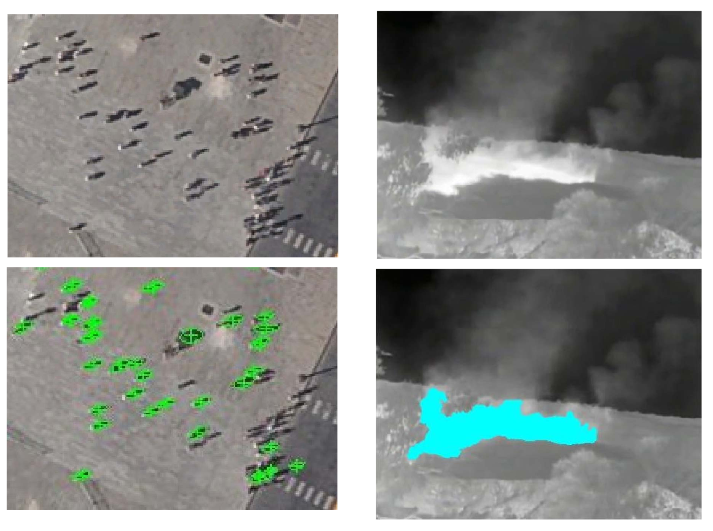
\includegraphics[width=12cm]{fire.png}
	\caption{Przykładowa detekcja ludzi (po lewej) i ognia \cite{FIRE}}
	\label{fig:fire}
\end{figure}

\subsection{Zadanie omijania przeszkód}

Systemy ostrzeżenia przed kolizją lub omijania przeszkód stają się powoli standardowym elementem wyposażenia dronów. Są one niezastąpione w sytuacji, gdy użytkownik traci maszynę z pola widzenia. 

Jedną z najczęściej rozważanych realizacji takiego systemu na platformach latających jest wykorzystanie stereowizji. 
Jej działanie polega na wyznaczeniu współrzędnych punktów sceny trójwymiarowej na podstawie obrazów uzyskiwanych za pomocą co najmniej dwóch kamer, co w efekcie umożliwia określenie odległości od przeszkód lub celów. 
Opisana w pracy \cite{STEREOVISION} implementacja algorytmu SGM (Semi-Global Matching) w układzie FPGA (XC7A100T) pozwoliła utworzyć mapę dysparycji w oparciu o obraz o parametrach $480\times 752$ @ $60$fps. 
Przetworzone dane są przechwytywane przez procesor wykorzystywany zazwyczaj w smartfonach (Samsung Exynos 4412 SoC) i zapisywane w pamięci DDR2. 
Praca ta została później wykorzystana na małej platformie UAV \cite{STEREOVISION2}, gdzie spełniała rolę systemu omijania przeszkód o niskiej latencji (poniżej $2$ms).
\begin{figure}[h]
	\centering
	\captionsetup{justification=centering,margin=1cm}
	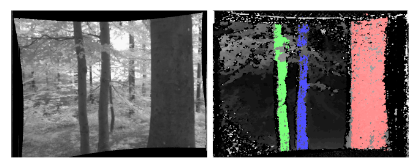
\includegraphics[width=13cm]{stereovision.png}
	\caption{System omijania przeszkód \cite{STEREOVISION2}. Po lewej wejściowy obraz w skali szarości, po prawej mapa dysparycji}
	\label{fig:stereovision}
\end{figure}

Kolejnym rozwiązaniem jest system detekcji linii zasilania \cite{STEREOVISION3}. 
W przypadku małych statków powietrznych, latających zazwyczaj na wysokości kilku, kilkunastu metrów, istnieje zwiększone ryzyko kolizji platformy UAV z instalacją elektryczną. 
Opracowany system wykorzystuje obraz stereowizyjny, poddając go równolegle transformacie Censusa oraz transformacji Top-Hat i określa stopień (koszt) dopasowania pomiędzy obrazami. %TODO 2 ale to chodzi o stereo -> tak wnoskuje.... %ODP Tak
Agregacja kosztów jest obliczana z uwzględnieniem obszaru wsparcia o krzyżowej postaci (eng. cross-based support region). %cross-based support region, nie mogłem znaleźć dobrego tłumaczenia
%TODO 2 - dac eng. %ODP OK
Po nieznacznej korekcie informacje są zapisywane w dwuportowej pamięci RAM i przekazywane do niezależnego procesora sygnałowego, który odpowiada za wyższą warstwę logiczną i realizuje funkcje decyzyjne.  
%TODO 2 - a doczytał Pan na jakies zasadzie to się dzieje ? %ODP w dokumencie nie opisano nic poza tym
Przetworzone informacje są ponownie przekazywane poprzez RAM do kontrolera wideo, który generuje obraz wyjściowy z wysegmentowanymi obszarami.
\begin{figure}[h]
	\centering
	\captionsetup{justification=centering,margin=1cm}
	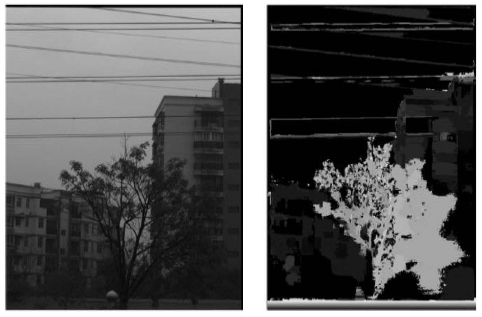
\includegraphics[width=12cm]{line_detection.png}
	\caption{Przykład systemu detekcji linii zasilania zrealizowanego w \cite{STEREOVISION3}. Po lewej wejściowy obraz, po prawej mapa dysparycji}
	\label{fig:line_detection}
\end{figure}

\subsection{Zadanie lokalizacji drona}
Inna praca \cite{Chenini} opisuje metodę estymacji pozycji drona w oparciu o obraz z kamery zamontowanej na statku powietrznym i skierowanej pionowo w dół. 
Pozwala ona wspomóc system nawigacyjny podczas lotu w utrudnionych warunkach (obniżających skuteczność np. GPS). 
Pierwszym krokiem jest określenie punktów zainteresowań -- wykorzystuje się w tym celu metodę Harrisa do wykrycia narożników, a następnie ZNCC (ang. Zero-mean Normalized Cross-Correlation) do określenia podobieństwa pomiędzy kolejnymi obrazami. %TODO 2 rozwinąć skrót ZNCC
Otrzymany zestaw informacji zawiera sporo nieprawidłowo skorelowanych par. 
Korekcja jest dokonywana w trakcie działania metody RANSAC (ang. Random Sample Consensus) opartej o algorytm Levenberga-Marquardta. %TODO 2 rozwinąć RANSAC i na tym bym skończył, bo co tu ma epipolarna do rzeczy ? %ODP OK
Implementacja systemu uwzględniała przeniesienie stworzonego wcześniej modelu programowego do części PS i stworzenie sprzętowego akceleratora dla detektora Harrisa. 
Wymiana informacji jest realizowana przez port ACP, który zapewnia bezpośredni dostęp do pamięci cache procesora. 
Ostatecznie, porównano sposoby implementacji detekcji narożników metodą Harrisa. 
Okazuje się, że dla podejścia programowego etap ten trwa ponad $750$ms, podczas gdy sprzętowa implementacja skraca ten czas do zaledwie $173$ms.

%TODO 2 - przegląd OK. Jakby się Panu udało w artykułach odszukać np. reprezentatywane zdjęcia i je tu zmieścic to już byłoby bardzo ekstra